\chapitre{Déontologie à gogo, le jeudi 21 juillet 2033 }{Ce qui, en temps normal, }{impressionne le plus Timothée et Shimoune quand ils viennent se caler, côte à côte, dans leur fauteuil de la salle du Conseil d’administration pour leur réunion mensuelle du Comité de déontologie de l’établissement (CDE), ce n’est pas la charretée de propos aussi doctes que biscornus, ni les yeux haineux de Philippe Flipper Dauphin, ni le regard impénétrable de Carl Michaud. Non, c’est le décor ambiant. C’est comme si les trois quarts de la masse budgétaire consentie à la décoration du CRG-BSL lors de sa construction avaient été affectés à la salle du CA. On se croirait à Balmoral, ce palais de la reine Victoria. Tout n’est que boiseries, caissons, frises, lustres, cuirs et tapis. De quoi séduire et rassurer n’importe quel banquier, n’importe quel politicien, n’importe quel philanthrope. }

S’il avait son mot à dire, le fils Tardif, il y a belle lurette qu’il aurait transformé la somptueuse pièce en bibliothèque classique, sombre, feutrée, sentant le bouquin poussiéreux, où, de temps à autre, entre deux décès survenus dans son parc à vieux, il irait se recueillir dans une méditation extatique, question d’oublier le caractère insoutenable de sa vie de Motté, de CS-1 du 5e Nord, d’enfant unique d’une Maririou saignante, blafarde, terrible. 

Paradoxalement, les trois carafes d’eau disposées sur la longue table semblent avoir été ramassées dans une vente-débarras et les verres sont en petit plastique cassant. Sur le mur du fond, immédiatement derrière le fauteuil du président d’assemblée, un cadre aux moulures XIXe représente le ministre Turcotte dans toute sa magnificence. Pourquoi pas une statue équestre devant l’entrée principale !

On devine que ce matin, Timothée a la tête bien loin des soucis bibliothéconomiques ou des aménagements de monuments. Non pas qu’il rumine, comme il le devrait, l’affaire Dart Vader Gagnon dont en haut lieu, on veut le coiffer. Il est plutôt aux premières lignes de ce désastre appréhendé dont le processus a été enclenché hier avant-midi par sa mère. Il n’a d’images que les draps souillés de sang, la pâleur de la possiblement cancéreuse Maririou et l’abominable commande du Dr Gagnon.

- Une chance que tous les Gagnon ne se ressemblent pas, pense-t-il un instant.

Pourtant, les deux risquent de lui faire perdre son boulot : l’un parce qu’il le force à voler des produits pharmaceutiques, l’autre parce qu’il a critiqué l’établissement dans les médias, ce qui est encore pire.

C’est à peine s’il suit le débat surréaliste portant sur la nature des soins qu’il est «administrativement possible» d’apporter aux pensionnaires en perte d’autonomie, ceux que l’on garde dans les salles 3P. Voilà des gens, pour la plupart, atteints de démence, de sénilité, de maladies incurables, des gens dont «les coûts d’entretien sont imprévisibles». Dans un contexte où les deniers sont rares, où la société doit financer ses universités, favoriser les études de pointe, aider la jeunesse talentueuse à acquérir les formations les plus pointues, a-t-on moralement le droit de dépenser des centaines de milliers de dollars sur une opération dont le bénéficiaire, un vieillard lourdement affaibli, un baby-boomer qui, sa vie durant, aura commis tous les excès, passera, de toute façon, en salle palliative (SP) quelques semaines plus tard ?

Sur un bout de papier, l’irrévérencieux Shimoune a dessiné un doigt d’honneur et le lui montre discrètement.

Quand un pensionnaire commence à souffrir de démence, pourquoi devrait-on lui fournir d’onéreux services ophtalmologiques, sachant que, de toute façon, elle ne lira plus de livres ou ne consultera plus de systèmes informatisés ? N’est-ce pas là du gaspillage ? Ou encore, pourquoi devrait-on sauver la prostate d’un octogénaire alité, le duodénum d’une vieillarde incontinente, l’ouïe d’une insomniaque médicamentée, la hanche d’une personne dépressive passant le plus clair de son temps couchée ?

Et de chuchoter son comparse :

- La queue d’un bande-mou ?

\begin{floatingfigure}[l]{40mm}

\includegraphics[height=60mm]{corps/chapitre8/img/personnage-timothee-jeune.jpg}
\end{floatingfigure}

Et la vie d’une vieille femme qui a des polypes endométriaux ou une tumeur peut-être cancéreuse, une vieille femme qui n’a pas encore été capable de dire «je t’aime» à quiconque, une vieille femme malgré tout attachante, doit-on la prolonger le plus longtemps possible afin qu’un jour, elle finisse par connaître la chaleur d’une relation affectueuse avec un fils lourdement perturbé ? Combien d’années de lucidité reste-t-il à cette femme brillante ? Dix ? Plus ? Moins ? Il y aurait tellement de choses à lui déclarer, à préciser, à expliquer, à se souvenir.

Se rappelle-t-elle de cette fête des Mères - Timothée devait avoir douze ou treize ans - où il était arrivé de l’école avec un important bricolage en papier gouaché, découpé, collé, broché, une carte de souhaits à rabats, sur laquelle il s’était appliqué toute la semaine ? Mais la pluie ayant créé des flaques de boue ici et là, le gamin s’était crotté les chaussures à la sortie de l’autobus scolaire et, en entrant avec son gage d’amour filial brandi à bout de bras, il avait souillé le plancher. Ce que voyant, la Maririou s’était mise à crier. Elle lui avait arraché la carte des mains, lui avait fait retirer ses galoches et l’avait enfermé dans sa chambre. Il n’avait jamais revu son œuvre et n’en avait plus jamais fait d’autres. Dans ses souvenirs, c’était la dernière fois qu’il avait tant pleuré. Perception d’enfant gravée à tout jamais au détriment des faits réels ? Allez savoir !

À son tour, Jacques Leblanc, un agent de recherche du ministère, économiste de formation se targuant de certaines connaissances actuarielles, se lève, et, de son dispositif personnel polyvalent (DPP), le modèle évolué et nécessairement corpo, projette des tableaux, des courbes, des boîtes couleur, où il est clairement démontré qu’à la grandeur du Québec, la durée moyenne de séjour dans les salles communautaires pour personnes en perte d’autonomie (SC3PA), c’est-à-dire les 3P, cas mineurs (3P-M) et lourds (3P-L) confondus, est de huit mois, treize jours et dix heures. Si c’est «nettement meilleur» que la moyenne canadienne qui est de neuf mois, vingt-deux jours et quatre heures, ce constat amène néanmoins une réflexion sur la «pertinence d’investir médicalement dans le contexte d’un tel état de fluidité».

- Les courbes de roulement que nous avons établies témoignent d’une dynamique très active et d’une constance remarquable; certaines provinces nous envient. Pour tout dire, nous pensons que ce serait jeter de l’argent à l’eau que d’augmenter l’enveloppe sanito curative, conclut-il.

- Sanito curative ? questionne le président d’assemblée.

- Euh, clinique, poursuit le fonctionnaire Leblanc.

Autrement dit, pourquoi rénover un appartement quand on sait que l’immeuble sera détruit dans huit mois ? Pourquoi voler des produits pharmaceutiques au profit du docteur Gagnon afin que Marie Rioux guérisse, une illégale qui a déjà un pied dans la tombe ?

- Ce n’est pas là dépenser les fonds publics de façon éclairée.

Le brillant exposé est terminé et quelques participants se dépêchent de féliciter l’orateur. Suit alors un silence qui frigorifie la pièce pourtant lourdement climatisée. Timothée se demande s’il ne serait pas possible, de nuit, d’arriver à faire monter un long tuyau galvanisé jusqu’au 5e Nord où l’on pomperait un peu de cet air rafraîchissant dans certaines salles, par exemple dans celle où sévit le tandem Thériault-Labbé, dans celle où repose Pierre Asselin ou même dans ce misérable coqueron de bureau qu’on lui a assigné.

- Mais ce sont des êtres humains, réfléchit un psychologue de pratique privée à la manière d’un camion qui frappe de plein fouet un pilier de béton.

Tiré de ses ruminations, Timothée est témoin d’une envolée implorant les considérations humanitaires et qui se termine sur une note plus politique.

- Cette génération a sûrement ses torts comportementaux, mais est-ce de sa faute ? Mérite-t-elle un tel châtiment ? Ne sont-ce pas les Boomers qui ont débarrassé le Québec de sa mythologie religieuse et qui en ont fait cette puissance économique respectée partout au Canada ?

Au lieu d’assister à une salve d’applaudissements, on entend plutôt la voix courroucée d’un «rouleur de r».

- Quelle mythologie rrreligieuse, s’insurge un médecin membre influent de l’église néo-évangéliste du Bas-Saint-Laurent. Si rrremplacer le Chrrrist et l’Évangile par la drrrogue, l’alcool et les maladies honteuses est pourrr vous un accomplissement, cette générrration mérrrite d’être enferrrmée au pain et à l’eau dans des salles en désorrrdre, leurrr élément de prrrédilection …

- Mange don’ d’la marde, interrompt Jipé Gendron, alias Tit-mononk, un pensionnaire en 2P qui représente les bénéficiaires sur ce comité.

Tandis que Philippe Dauphin prend des notes, ses yeux noirs sur cet émule de Dart Vader, l’avocat Rémi Anglehart, président d’assemblée et conseiller juridique de l’établissement, se dépêche d’intervenir.

- Messieurs, messieurs ! On se calme. On ne quitte pas cette harmonieuse civilité qui nous caractérise.

- J’ai fait mon point, conclut néanmoins le médecin rrrouleur, ce qui oblige Tit-mononk Gendron à avoir le dernier mot :

- Crétin !

Puis devisant l’économiste :

- As-tu fait des calculs pour savoir combien de vieux de plus, tu pourrais rentrer dans les centres en réduisant d’un pied la largeur des lits ? Ou en les mettant à deux étages, les incontinents en bas, les propres en haut ? Et pour sauver, tu pourrais couper de moitié le nombre des matelas : on aurait un jour «avec matelas» et un jour «sans». Tant qu’à y être, pourquoi tu leur dis pas, à tes boss, de rendre obligatoire partout le projet du Dr Bellavance. Au moins là, on pourrait devenir rentables, nous autres les vieux ! Crétin !

- Monsieur Gendron, s’il vous plaît !

- J’ai pas fini de parler, Anglehart, ‘sti ! T’auras rien qu’à m’envoyer rejoindre Dart Vader dans vos geôles du sous-sol, chez les Papyblues !

Les traits de Carl Michaud se contractent au point de ressembler à ceux de Flipper.

- Les générations X et Y reprochent aux baby-boomers de ne pas avoir fait assez d’enfants, poursuit le bonhomme. Mais quand je vous vois, toute votre gang de crabes en train de calculer combien de grammes de manger mou vous pouvez nous chipoter pour mieux équilibrer vos sacraments de budgets, je pense que les baby-boomers en ont fait beaucoup trop d’enfants. Ils auraient dû tous faire comme moi, se faire vasectomiser à 28 ans !
Me Anglegart commence à s’échauffer.

- Monsieur Gendron, vous vous emportez et ça n’avance en rien le débat.

- Point d’ordre, monsieur le président, le représentant des bénéficiaires nous fait perdre inutilement du temps ! Après ça on se demande pourquoi des gens de mon âge traitent de «vieux dégénérés» certains spécimens – il pointe vers Tit-mononk - de cette génération !

C’est un jeune homme à la mine fort grave, le délégué du Conseil de développement économique régional, qui a parlé.

- M’a t’en faire des «vieux dégénérés» p’tit fasciste néolibéral ! rétorque aussitôt le vieillard.

L’officiant ès procédure s’étire les bras. Il est sur le point de perdre le contrôle.

Noblesse oblige, c’est Carl Michaud, le DG, qui le tire immédiatement d’affaire. Il a levé un doigt.

- La parole est à monsieur Michaud, notre bon directeur général, prononce nerveusement le président par-dessus le tohu-bohu.

Une main en l’air, il se retourne vers Claude Sey, un jeune rédacteur au service de la direction des communications qui fait office de secrétaire d’assemblée.

- Monsieur le secrétaire, veuillez ne pas considérer dans le compte-rendu, les échanges impliquant M. Gendron.

- J’efface tout ?

- Tout. Je m’en porte responsable, précise l’avocat en faisant un signe de tête au grand patron.

Tous se taisent. Carl Michaud a pris la parole.

- J’aimerais demander au représentant des chefs de section, ces professionnels qui sont en contact direct et quotidien avec nos bénéficiaires dans les salles communautaires pour personnes en perte d’autonomie, les 3P, ce qu’il pense de la question, à savoir, la nature des soins qu’il est administrativement possible d’apporter à ces pensionnaires mal en point. Qu’en dites-vous, monsieur Tardif ?

Horreur consommée ! Voilà la punition que le patron a décidé de lui infliger : prendre la parole devant une longue tablée de bonzes, de médecins, d’avocats, d’administrateurs, d’ingénieurs, d’économistes ! Lui qui n’a qu’un certificat d’études collégiales. Lui qui n’est qu’un Motté rase-mur qui ne voit que les godasses des autres, qui ne perçoit que leur choc, plus ou moins amorti selon les personnalités, sur le plancher ! Lui cet être de toutes les timidités, ce fils écrasé par une tyrannique marâtre, ce mauvais joueur de trombone, instrument exécré, cet employé victime de toutes les moqueries, ce petit technicien sans panache, ce binoclard de plus en plus chauve détestant son image. Sûrement que le soupçonnant d’inconfort extrême en public et de vacuum cérébral, Carl Michaud, ce salaud fringué en président de banque, a choisi de l’humilier. C’est de cette cruelle façon qu’il lui fera expier la gaffe majeure de Dart Vader ! À preuve le sourire sadique de Dauphin.

En vérité, jamais Timothée ne s’est retrouvé dans une telle situation. Épouvanté, il lorgne un instant Saint-Pierre qui semble l’encourager d’un signe de tête. De deux choses l’une : soit il balbutie une insipidité, auquel cas il passe pour ce qu’on croit qu’il est et le DG se venge, soit il livre, à sa manière, le fond de sa pensée, auquel cas, bon Dieu de bon Dieu, il surprend et il vit avec les conséquences. Des conséquences sûrement négatives ! La Maririou, elle ? Seigneur ! Elle serait déjà en train d’articuler sa façon de penser à grand renfort de coups de paume sur la table.

Shimoune lui refait un signe de tête, cette fois, les sourcils en accent circonflexe.

Timothée se décide de sauter.

- Je ne suis pas un grand parleur, se lance-t-il avec une voix saccadée tout embarrassée de tremblements inconfortables, une voix qui a trop peu parlé dans sa vie. Est-ce que j’ai bien compris votre question ? Vous voulez entendre le point de vue de quelqu’un qui passe le plus clair de son temps avec les bénéficiaires les plus mal en point ?

Carl Michaud opine des yeux.

- Bon, OK !

Plus mort que vif, le CS-1 boit une gorgée d’eau.

- Euh … je suis quelqu’un qui a de la misère avec les phrases compliquées et les concepts trop savants; je vais plutôt vous présenter un exemple parmi bien d’autres, un exemple qui, comme on dit, vaut mille mots. Euh … ici au CRG, on a, comme vous savez, un système de gestion informatique plein de bogues, ce qui nous fait perdre beaucoup de temps et qui doit coûter très cher.

Le DG a pris le fixe et Shimoune Saint-Pierre a cessé de respirer.

- Mais il s’adonne que depuis quelques mois, poursuit Timothée l’adrénaline commençant à le propulser, j’ai dans ma salle 3P-M un ingénieur informatique de 83 ans qui a encore toute sa tête. Ce gars-là, toute sa vie, il a installé des progiciels de gestion, des machins SAP, Microsoft, ou bien des grosses patentes compliquées comme ici. Il a pris sa retraite il y a sept ans et, quatre ans plus tard, on l’a accueilli ici parce que ses enfants lui avaient volé toutes ses économies. Il est en train de devenir aveugle parce que vous ne voulez pas l’opérer, parce que ça coûte trop cher, que ça serait contre-productif. Il maigrit de jour en jour parce qu’il déteste le Nutrisuz et qu’on n’a pas le droit de lui donner quoi que ce soit d’autre. Il est dépressif parce qu’il ne peut plus lire ni voir de films ni aller au théâtre, ses passe-temps préférés. Il n’a que moi à qui parler, parce que j’ai une petit certificat en informatique et que j’accepte d’oublier un petit peu le règlement qui interdit la fraternisation avec les bénéficiaires. Il est triste parce que ses voisins, des vieux aussi poqués que lui, n’arrivent pas à le piffer. Faut admettre qu’il est un peu spécial, mais, bon, ça, c’est une autre histoire.

Le délégué du Conseil régional des maires a manifesté un peu d’impatience et Flipper Dauphin prend frénétiquement des notes.

- Pourquoi je vous parle de lui ? Parce que je sais que si vous vouliez le remettre sur pieds, mon monsieur, il saurait probablement vous réparer et faire fonctionner votre système de gestion; il en a vu des pires. Il a même une bonne idée de la cause du problème. En tout cas, c’est ce qu’il m’a dit. Peut-être que ça lui redonnerait le goût de vivre, peut-être que dans sa tête, tout ça - Timothée a fait un grand geste circulaire - serait soudainement devenu logique. Et peut-être que ses habiletés pourraient vous tirer d’affaire. Mais dépêchez-vous, je suis à la veille de le transférer en 3P-L, si ce n’est pas en SP. À vue de nez, il est PPLH.

Il a fini de parler et il regarde sa feuille griffonnée en avant de lui. Me Anglehart se désenrhume.

- Qu’entendez-vous, monsieur Tardif, par PPLH ?

- Passera pas l’hiver !

Et le silence de frapper la salle à nouveau. Pesant.

- Comment sait-il qu’il pourrait réparer notre système ? demande enfin le DG.

- Il a déjà vécu une situation semblable. Je lui ai montré le système. Il est venu dans mon bureau. Pas longtemps, mais juste assez pour qu’il voie.

Vlado Markovsky, le très éprouvé directeur de l’informatique, s‘insurge.

- Vous n’aviez pas le droit de faire ça ! siffle-t-il, le coin des yeux rivés sur Carl Michaud.

L’intervention a l’heur de démarrer un bal de messes basses et Me Anglehart doit lancer deux appels à l’ordre pour que Carl Michaud puisse reprendre la parole.

- Continuez, monsieur Tardif !

- Dans son cas, à mon ingénieur, les processeurs sur le site où il devait implanter une solution SUSE 256 avaient été tatoués pour ne pouvoir fonctionner correctement qu’avec l’option Microsoft. Une histoire de pot de vin qui avait fini par coûter très cher au client …

La fin de sa phrase se perd dans une cacophonie où le président Anglehart se retrouve impuissant à ramener l’ordre. Carl Michaud doit frapper la table de ses deux mains. Le calme revenu, la situation informatique est déclarée étrangère à l’ordre du jour et la discussion peut continuer sur la déontologie comme si le représentant des chefs de section n’avait pas parlé. Finalement, comme il est d’usage en de tels forums, le gros bon sens est incapable de faire le poids avec toutes ces idées pontifiées avec méthode, influence et soutien audiovisuel. Car une fois lancées, ces importantes billevesées deviennent généralement immuables et seul un rapport de force suffisant peut arriver à en débarrasser l’assemblée. Ce n’est évidemment pas le cas en cette 42e session du CDE et, trois quarts d’heure plus tard, Timothée quitte la réunion aussi perdu de stress et de peine qu’il ne l’était à son arrivée.

Mais Carl Michaud, lui fait signe.

- Ton chien est mort, Momo, lui grince son ami. C’est maintenant qu’il va te bouffer tout cru !

Livide, Timothée s’approche quand même du DG.

- Monsieur Tardif, j’entends aller, le plus tôt possible, parler avec votre pensionnaire. Pourriez-vous m’arranger le coup ? J’aimerais cependant que cela reste, disons, à caractère privé.

Ce que voyant, Vlado Markovsky quitte la pièce, l’œil sombre. En tant que grand manitou des TI, il vit un cauchemar depuis quelque temps. Il a beau savoir que la faute incombe aux gens de l’ACRG (Association des centres régionaux de gériatrie) qui ont imposé cette plate-forme SUSE 256 pour faire tourner le progiciel de gestion et que dans cette calembredaine haut de gamme, il peut effectivement y avoir eu tatouage de puces. C’est pourtant lui qui, localement, est pointé du doigt à chaque fois que le système plante. Et là, on va lui mettre un vieux schnock dans les jambes, un ingénieur grabataire avec qui il va devoir composer, qui va peut-être, lui, repérer la cause véritable du problème. Comme si ce n’était pas assez compliqué ! Tout cela à cause de ce mal dégrossi de Tardif. Un Tardif qui, pas plus tard qu’hier en matinée, est venu lui ravir le Dr Gagnon pour une urgence, soi-disant, au moment où lui, cadre supérieur du CRG-BSL, il était sur le point d’accéder au cabinet du bon docteur à cause de son problème de stress. Pour cette raison, il a dû se dénicher un nouveau rendez-vous et rentrer bredouille au Centre. Mais au fait, qu’est-ce qu’un vulgaire CS-1 peu argenté faisait avec une situation d’urgence entre les mains, chez un médecin privé, pendant les heures d’ouvrage, alors qu’il y a des médecins en permanence au Centre ? N’était-ce pas là une histoire à odeur de soufre? Ne serait-il pas de son devoir d’en informer quelqu’un mieux outillé que lui pour faire enquête ? À quelqu’un comme cet inquiétant Dauphin qui est toujours à trotter dans le sillage de Carl Michaud ?

Au même moment, Sey, le secrétaire d’assemblée, rejoint Timothée et Shimoune dans le couloir.

- Très bien parlé, monsieur Tardif. Vous avez fait la preuve qu’il était possible d’œuvrer dans une boîte comme celle-ci sans s’être remplacé le cœur par une roche gavée de circuits imprimés.

- Par contre, il a dû se faire quelques ennemis, le Momo, grince Shimoune en produisant un geste ignoble.

- Ça, c’est sûr. Mais si jamais je peux être utile, faut pas hésiter à me contacter.

Shimoune le regarde alors très sérieusement.

- Tu travailles pour le Flipper, non ?

- Oui, mais ça veut pas dire grand-chose, croyez-moi.

Vers 13 h, Timothée qui a vraiment envie d’être à des kilomètres du Centre, roule bruyamment en direction de son officine. Mais voilà qu’en passant devant le poste de garde, il surprend une nouvelle altercation entre le père Martel et Laurent Bérubé. Cette fois, il n’est pas question d’alcool, mais de la «petite chambre». Véritable secret de Polichinelle, ce local exigu équipé d’une cuvette et d’un lavabo, mais qui n’a qu’un petit lit pour tout mobilier, sert de lieu de rencontre pour les couples hétérosexuels hébergés, bien malgré eux, en 2P, l’une chez les dames, l’autre chez les hommes. De cette façon, ils peuvent, de temps à autre, se retrouver pour s’offrir de doux moments d’intimité. Même si moins de 20 % des pensionnaires se prévalent de cette largesse officieuse, l’achalandage est surprenant. Certains vieux complices se débrouillent même pour y passer des nuits. Encore ici, le truc est de s’assurer monétairement de la complicité des proposés aux bénéficiaires, une modalité que ne semble pas avoir comprise le père Martel.

- C’était à mon tour, à soir, et il a donné ma place à un autre, rage-t-il.

Timothée observe la réaction de Laurent qui hausse les épaules en signe d’impuissance.

- T’es certain qu’y a rien à faire ?

- Faudra voir avec Ronnie. C’est lui qui me remplace à 16 h.

Or Ronnie Ross était encore plus véreux.

- Qui occupe la petite chambre, ce soir ?

Au lieu de répondre, Bérubé hausse à nouveau les épaules. Timothée qui en a sur le cœur plus qu’il ne peut en supporter, hausse alors le ton, un phénomène inédit au CRG-BSL. Lui-même n’arrive pas à croire ce qui lui arrive.

- Laurent, je t’ai posé une question très simple : qui occupe la câlisse de p‘tite chambre, à soir !

- J’sais pas, gronde le sous-fifre. C’est Ronnie qui a la liste.

Dès lors, le CS-1 double tape sa boucle d’oreille.

- Ronnie Ross, commande-t-il.

Au bout de quelques secondes, une voix finit par se faire entendre.

- Allô ?

- Ronnie ?

- Ouais ! C’est qui ?

- Timothée Tardif. J’ai une question.

- OK le Motté. Shoot !

- Qui est censé passer la soirée dans la p‘tite chambre, aujourd’hui ?

- Aujourd’hui ? Personne. J’ai rien sur ma liste. Ça va à demain après-midi.

- C’est beau. Quand tu entreras à 16 h, veux-tu noter que monsieur Martel et sa femme vont y passer la nuit ?

- Pas de problème, je vas les ajouter !

L’appel complété, Timothée explique calmement au vieillard qu’il lui est maintenant loisible d’aller occuper le galetas nuptial où il pourra demeurer un bon 24 heures s’il le souhaite. Ce qu’entendant, le bonhomme disparaît n’en croyant pas sa bonne fortune. De son côté, puisqu’il est intelligent, Laurent Bérubé ne dit rien. Il attend l’imprévisible; le Motté a en effet levé le ton et s’est mis le nez dans une combine qui marchait bien. Voilà qui est inédit. Mais au lieu d’une admonestation en règle, il a droit à l’articulation d’une promesse, un engagement que le chef de section émet sèchement en direction du plafond et du comptoir:

- Un jour, j’vas sacrer mon camp loin de tout ce crossage de monde, de toute cette magouille inhumaine, de tout ce mépris au plus fort la poche ! Et ce jour-là, plus ça va, plus il approche ! Je vais m’en aller dans un endroit où je vais pouvoir porter mon prénom au complet, la tête bien haute, sans que personne ne vienne rire de moi.

Il n’a pas parlé, pas plus qu’il n’a crié ou pleuré. Il a simplement expulsé de son système, tels d’abominables miasmes, humeurs et autres déchets, une sourde rancœur basée, à ce qu’il semble, sur la seule certitude dont il disposait pour l’instant, celle d’une lumière blafarde qui commençait apparemment à poindre quelque part, pas trop loin, en avant de lui.

Et dans ce maigre début de clarté, il n’y avait plus de CRG-BSL de merde, plus de Ronnie Ross, plus de Carl Michaud, plus d’illégaux, plus de gros Turcotte.

Décontenancé, Bérubé file vers n’importe où comme il sait si bien le faire. Quant à son chef, il met le cap sur la pizzeria voisine du Centre, la bien nommée Da Peperone, où, plus tôt dans la journée, lui et Shimoune avaient convenu de se rencontrer peu après 14 h.

Pourtant, juste avant de quitter, il aperçoit - c’en est devenu une habitude - Luce Morency qui longe le passage, appuyée sur la rampe murale. Elle s’est encore échappée. Si ça continue, les gens du 6e vont devoir l’envoyer en salle palliative ou bien ils vont la maintenir attachée dans son lit en 3P-L. Et pourquoi, diable, est-ce toujours sur lui que ça tombe ? Sans rien brusquer, il stoppe sa souffreteuse Saguewanish, la cale le long du mur et prend la main de la vieille dame.

Du plus profond de sa démence, elle le regarde.

- On se connaît ?

- Venez madame Morency, on va s’asseoir là-bas sur les chaises.

Il se pince la boucle d’oreille :

- 6 Nord, code Magenta !

- T’as trouvé la mére Morency ? demande la voix. Elle a-t-y du linge ?

- Comme d’habitude, répond Timothée, sans oser trop regarder.

- OK, on y va !

En dirigeant la vieillarde vers les inconfortables fauteuils, Timothée lui parle, tout doucement, de l’été 1996 au lac Saint-Mathieu, «la fois que les eaux du lac avaient monté».

- J’avais failli me noyer; c’est une petite fille de Montréal qui m’avait sorti de l’eau.

- Le lac …

- Je me souviens même plus d’elle, de cette petite fille qui m’avait empêché de caler …

- Madame, madame ! avait crié la gamine à cette belle femme qui prenait le soleil devant sa brinquebalante roulotte louée. Vot’ tit-gars a failli se noyer !

Étendue en bikini sur une chaise longue en treillis de plastique jaune et blanc, la Maririou s’était levée et, se mordant le poing, s’était mise à courir, on l’aurait dit affolée, vers les deux enfants. Sans remercier la fillette, elle s’était emparée de Timothée et l’avait ramené à la maison mobile, le tenant par la main comme s’il eut s’agit d’une chiffe molle. À l’intérieur, sans hésiter un seul instant, elle lui avait administré une sérieuse fessée.

- Espèce d’innocent, me faire un coup pareil !

Le bambin avait été puni trois jours. Trois jours pendant lesquels il n’avait pas eu le droit d’aller à plus de cinq mètres de la roulotte alors que tous les autres enfants passaient leurs journées à s’amuser dans l’eau où sur ce qui restait de grève à la suite de la crue anormale. Il avait été puni pas parce qu’il aurait pu perdre la vie, mais parce que, ce faisant, il aurait pu faire beaucoup de peine à sa mère. C’était donc la preuve alambiquée qu’elle l’aimait. Et elle l’aimait peut-être encore, en ce début d’après-midi, dans son lit de malade, dans son lit d’octogénaire très malade.

Luce Morency regarde Timothée avec attention, comme si cette anecdote lui rappelait quelque chose. Un instant, elle revoit un chemin tout en croches, en montées et en descentes, avec sur chaque côté, des champs pleins de fleurs, des champs tout en buttes, avec des clôtures en pagées de cèdre, des chiens qui sautent dans les foins, des corneilles, des abeilles. Le rang menant à Trois-Pistoles ? Mais elle n’ouvre pas la bouche, elle ne sait plus. De toute façon, le gros Lavoie, ce salaud, vient d’arriver avec un fauteuil roulant et une couverture.

- Là-là, ça va faire, la mére, qu’il lui dit en la couvrant. J’vas vous attacher dans votre lit, avez-vous compris ?
Il aide la démente à s’asseoir et, sans un mot pour Timothée, disparaît avec elle dans l’ascenseur. Il paraîtrait que Luce Morency ne souffre pas de la maladie d’Alzheimer, un fléau que les chercheurs ont fini par «contrôler» – à défaut de pouvoir dire «éradiquer» - au tournant des années 20. Désormais, les vieux reçoivent un vaccin et ils peuvent «survivre», pour ce que ce mot veut dire, avec toute leur mémoire. Pourtant, il semble y avoir de plus en plus de cas de démence comme celui de madame Morency. Y aurait-il un rapport ? Allez savoir !

- Tu t’es fait une blonde, le Motté ?, lui lance, clin d’œil à l’appui, le père Jean qui s’adonne à traîner ses misérables savates par là.

- S’il vous plaît, monsieur Jean …

Mais l’inutile phrase s’arrête là et le CS-1 file vers l’ascenseur.

Il va s’en aller rejoindre Shimoune au Da Peperone et il va tout lui raconter. Tout ! Même l’épisode du docteur Gagnon. Surtout celui-là ! Peut-être va-t-il déborder sur Louis-Marc Richard et l’énorme probabilité de délation que ce salopard laisse appréhender. Peut-être va-t-il s’épancher sur son existence de fils misérable, une vie sans affection et, surtout, pleine d’ennuis, de gros ennuis, une vie où les joueurs de lyre sont dans les livres anciens. Peut-être que Shimoune va l’écouter sans rire, sans être méchant, peut-être qu’il va lui donner son avis, un conseil, et peut-être qu’il va lui apporter une forme d’aide.

Chemin faisant, Timothée croise son épouvantable collègue responsable du 4e Sud, un certain Pierre Monger, dont l’ouverture d‘esprit n’a d’égale que la qualité de ses amis, le plus connu étant le gros Lavoie. On dit que tous deux seraient, en quelque sorte, les principaux piliers de la mafia qui sévit au CRG-BSL. L’œil narquois, le sinistre personnage lui passe une remarque sur le comportement anormal de sa bécane. Mais l’autre choisit d’ignorer et de continuer sa bruyante chevauchée vers le resto. Il est inutile de se mettre cet immonde porc à dos plus qu’il n’en faut. Qui sait, peut-être aura-t-il besoin de lui et du gros Lavoie pour se procurer les produits pharmaceutiques du Dr Gagnon ? Ces malfrats ont sûrement une combine.

Avec cette pensée en tête, il entre dans le boui-boui où il retrouve Saint-Pierre occupé à dévorer sa pointe de pizza mexicaine. Comment fait-il pour manger une telle horreur ?

- P’is mon Momo, t’as affaire à moi ? T’es-tu tanné d’être straight ?

Timothée déteste se faire appeler ainsi en public.

- Non mais j’ai besoin de tes conseils sur deux points.

- OK ! The Doctor is in ! Je t’écoute.

Dans un premier temps, comme pour se réchauffer en tournant autour du pot, le pauvre hère relate son expérience holographique ainsi que la conclusion romantique survenue l’avant-veille au soir.

- Je pense que je sais c’est qui, la fille, mais je n’ai pas ta pratique des fréquentations, même si dans ton cas elles sont «douteuses». Je ne sais plus quoi faire. J’ai besoin d’un conseil.

- C’est qui, d’après toi ?

Quand Timothée mentionne le nom de Marie-Odile Tremblay, Shimoune ne peut retenir l’explosion d’un grand rire venu de l’abdomen, plein de spasmes et de larmes.

- Tu viens de faire ma journée, Momo, soupire-t-il. Si c’est ça être straight, maudit que je suis content d’être gai !
Il n’en fallait pas tant pour que l’atmosphère s’alourdisse.

- Si j’avais voulu faire rire de moi, je serais resté au Centre; je ne serais pas venu ici !

- Je m’excuse, ç’a été plus fort que moi. Mon conseil ? Si c’est bien elle, ta bonne femme, fous le camp, cache-toi au plus creux des sous-sols, au plus profond des bois, prend le large, ne la laisse pas t’approcher. Elle est vraiment vicelarde ! C’est une coriace, une sale flic, un cafard !

Voyant l’heure avancer, Timothée décide d’accélérer, quitte à tout perdre. De toute façon, il ne sait plus à quel saint se vouer. Alors, il plonge et, en moins de deux minutes, raconte tout : ses parents, sa mère, l’hémorragie, le docteur Gagnon, les produits pharmaceutiques, la surveillance électronique. La totale !

- Wow, tu tripes fort !

- Je sais pas par quel bout prendre ça.

Pour Shimoune Saint-Pierre, il n’y a pas trente-six solutions. Ou bien Timothée livre ses vieux aux limiers du BAG, ce qui va à l’encontre de toute logique et qui, pour l’instant, est inconcevable. Ou bien il fait disparaître le docteur Gagnon, ce qui est un assassinat venant complexifier lourdement l’affaire. Ou bien il neutralise ce profiteur, ce qui l’oblige à faire enquête et à ramasser des preuves contre lui, ce qui prendrait beaucoup trop de temps. Ou bien il a recours à des écumeurs comme le tandem Monger-Lavoie, ce qui risque de lui coûter encore plus cher tant ces malfaiteurs sont voraces. Ou bien il s’outille pour défoncer le centre nutritionnel de nuit, ce qui, advenant que le coup réussisse, le force à disparaître pour toujours. Ou bien il se sert de sa tête.

- Qu’est-ce que tu veux dire ?

- Réfléchis un peu. Quel est ton principal obstacle si tu veux voler des médicaments ?

- La surveillance électronique.

- Et qui contrôle la surveillance électronique ?

Son interlocuteur n’ose répondre.

- T’as tout compris. Marie-Odile Tremblay, celle-là même dont on parlait tantôt. C’est elle la clé de ton problème.
Dès ce moment, tout va se mettre à s’accélérer et le lointain horizon à s’éclairer encore un peu.

En s’en retournant au Centre, Timothée apprend par téléphone que le docteur Gagnon est passé avec ses appareils et que la Maririou n’avait pas de tumeur. Il a pu lui enlever ses polypes par chirurgie hystéroscopique. Elle a donc été stabilisée, mais elle doit dormir beaucoup et Gagnon lui a donné des kilos de médicaments à avaler. L’ardoise est donc en train de s’allonger.

Arrivé au 5e Nord, il s’enferme dans son officine où il tourne en rond comme un perdu, comme s’il y avait une trombe emprisonnée dans la tête, une tornade qui voulait lui arracher toutes les synapses. Gagnon en est à sa deuxième visite, il a pratiqué une intervention, il a laissé sur place une impressionnante pharmacopée, la Maririou n’est pas tirée d’affaire pour autant, il y aura peut-être des complications, elle a 82 ans et ça pourra être long, très long. La dette sera fabuleuse. Or, dans ce cauchemar, ce pourrait être Marie-Odile Tremblay qui serait «la clé», c’est-à-dire qui pourrait agir comme «ouverture» vers une solution ! Auquel cas, comment procéder pour mettre la main sur cette fichue clé ? Réalisant qu’il était sur le point de sombrer dans une crise d’angoisse, Timothée décide d’aller raconter son drame à Robespierre, l’héritier spirituel de l’inventeur du Pétépano. Le gars est fiable, il est ouvert à vouloir l’aider et voit déjà un peu clair dans cette histoire tordue. À coup sûr, il l’écoutera et le conseillera sur Marie-Odile. Ne semble-t-il pas la connaître ?

Mais à mi-chemin, couic ! crac ! euffh!, sa trottinette meurt brusquement de sa belle mort, une mort annoncée, mécanique, détestable. Timothée doit donc rebrousser chemin et traîner son véhicule jusqu’à son bureau. Le voyant ainsi démonté, le père Martel accourt et, prétextant vouloir regarder la carcasse de plus près, fait un signe discret à Timothée.

- C’est le bonhomme Jean qui a saboté votre bécane, tout le monde l’a vu faire. Avant, il travaillait comme mécanicien à l’usine Saguewanish au Lac Saint-Jean. Fait que …

- Tout le monde l’a vu ?

- Ben, mettons quelques-uns, entre autres, les joueux de 500.

- Madame Bellow ?

- Non, pas elle. Elle n’était pas là.

- Merci, monsieur Martel.

Le temps de chasser l’image de ces vieux auprès de qui il est un des seuls à être respectueux, poli et serviable, mais qui, pourtant, ont laissé le bonhomme Jean lui saboter sa Saguewanish sans lever le petit doigt, sa boucle d’oreille lui agace l’oreille à nouveau, l’empêchant de téléphoner à l’atelier mécanique.

- Timothée Tardif !

- Allô, c’est Claude Sey !

- Ah ! Rebonjour!

Je suis en mode confidentiel.

- Attendez. OK. Moi de même.

Timothée a appuyé sur un petit bouton à l’extrémité de son appareil.

- Flipper va faire enquête sur vous. Une histoire de médecin que vous êtes allé chercher d’urgence à sa clinique privée hier avant-midi !

- Ah …

- Il trouve qu’il y a anguille sous roche. Et comme il vous en veut, ben …

- Ah …

- C’est Markovsky qui lui a raconté votre histoire, un autre qui vous en veut ….

- Ah …

- À votre place, je bougerais vite !

- Merci !

Dieu du ciel, est-ce que ça va s’arrêter quelque part ?

On dirait, parfois, que les scénarios qu’offre la vie sont aussi alambiqués que ceux que pondent les pires scénaristes d’Hollywood. Cependant, il arrive que les agencements grossiers de faits improbables soient la norme. Auquel cas, l’impensable finit par couler de source. On entend souvent quelqu’un dire qu’il ne pourrait jamais faire un film à partir d’une séquence réelle de son vécu parce que tout le monde décrocherait tant l’histoire semblerait «arrangée avec le gars des vues». C’est pourtant un tel caprice du sort qui attend Timothée.

Quand, quinze minutes plus tard, après avoir traîné sa bécane jusqu’à l’atelier de réparations, il marche en direction de sa voiture tout au fond de l’aire réservée aux véhicules à essence - les zones les plus proches des accès au Centre sont toutes dédiées aux bagnoles électriques – il tombe sur Sébastien Larose, assis la porte ouverte, dans sa Subaru hybride.

- Salut mon homme, fait ce dernier.

Timothée lui répond d’un bref signe de tête.

- Je cherche encore un mot !

- Ah !

- Un mot de dix lettres qui signifie «aide extérieure au bon roulement dans les soins de santé». Je suis pas sûr de comprendre.

- Dix lettres ?

- Pis la 3e et la 4e lettre, c’est TH et, plus loin, y a un N …

Timothée se gratte le crâne.

- EUTHANASIE !

- EUTHANASIE ?

- Ouin, fait-il en continuant vers sa voiture, étincelante de soleil deux espaces plus loin.

- Eh ! Ça marche ! T’es pas pire, mon homme !

Arrivé à sa bagnole, il remarque qu’elle semble débalancée, comme si elle était penchée vers la droite. Une rapide inspection lui permet de constater que les deux pneus du côté passager sont à plat. On les a crevés, troués, vandalisés. Comme sa Saguewanish. Cela pour lui rappeler qu’on le détestait, qu’il était un déchet, un Motté, qu’on le voudrait ailleurs qu’au CRG-BSL, qu’il était laid, bedonnant, binoclard, sans blonde et en voie d’être chauve, qu’il jouait du trombone et que sa mère était une vilaine Maririou.

Telle une puissante nausée, un sentiment profond de découragement s’empare de lui.

- Pourquoi, pourquoi, pourquoi, maudite misère, crie le pauvre diable sans s’en rendre vraiment compte. Ça va-t-y finir un jour par finir, câlisse ?

L’imprécation a attiré l’attention de Larose.

- T’as un problème, mon homme ?

- Ils m’ont crevé mes pneus ! J’suis plus capable, moi ! Faut que ça arrête !

On aurait dit un sanglot. Ce que jugeant, Larose adopte automatiquement son visage des grands jours. Du temps où les affaires allaient bon train.

- Fais un rapport tout de suite. C’est le Centre qui est responsable de la sécurité dans le stationnement. Y vont faire une enquête et s’ils concluent qu’il y a eu vandalisme, ils vont te rembourser. Niaise pas avec ça !

Dans un tout autre contexte, Timothée aurait pu trouver la suggestion intéressante. Mais il semble prostré, incapable de faire quoi que ce soit. Son compagnon décide donc de se taper la boucle d’oreille et d’appeler la Sécu.

- On envoie quelqu’un, restez sur place ! entend-il.

\begin{floatingfigure}[l]{40mm}
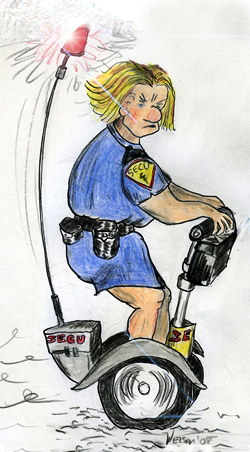
\includegraphics[height=60mm]{corps/chapitre8/img/personnage-marie-odile.jpg}
\end{floatingfigure}

C’est ainsi, étrange rebondissement, que Marie-Odile Tremblay, la Bitch elle-même, arrive, deux minutes plus tard, sur un Saguewanish orné d’un phare gyroscopique brandi à bout de tige. Dès lors, c’est le syndiqué qui explique la situation, en ajoutant que Timothée ne peut plus rouler, qu’il en a assez de ces vexations gratuites et qu’il a vraiment envie de porter plainte.

Sérieuse comme une statue médiévale, Marie-Odile fait méticuleusement le tour de la voiture sinistrée, entre un crayon dans les trous pratiqués aux pneus de droite, enregistre un clip vidéo et dicte quelques notes à sa boucle d’oreille.

- On va la faire remorquer au garage que vous voulez, dit-elle, et, de là, vous pourrez vous en occuper.

Le CS-1 accepte et l’opération est organisée illico. Que va-t-il faire maintenant ? Il est presque 17 h et son père l’attend.

Elle l’a vu regarder sa montre.

- Pour moi aussi, c’est l’heure; je viens de finir mon quart de travail.

- Ah …

- Je peux vous … te déposer où tu veux; mon auto est juste là !

En temps normal, Timothée n’en aurait cru ni ses yeux, ni ses oreilles. Il aurait plutôt estimé avoir gagné à la loterie. Mais cette après-midi, plus rien ne l’étonne. Il est devenu un brin d’herbe que le vent emporte à sa guise. Il n’a plus prise sur cette réalité si laide. Sa mère, le docteur Gagnon, Louis-Marc Richard, Dart Vader, Flipper Dauphin, le DG, Marcovsky, Bérubé, le Gros Lavoie, le père Jean, sa Saguewanish, ses pneus ! Comment supporter sans craquer autant de mauvaises nouvelles, de désagréments, de haine, de drames ?

D’un signe de tête, sans même esquisser un sourire, les yeux presque invisibles derrière ses épaisses lunettes, il accepte l’offre. Alors, contre toute attente, Marie-Odile l’informe qu’elle va le déposer chez lui à Nazareth. Autant en emporte le vent ! Incapable de parler, il acquiesce d’un geste imperceptible. Le regard vers la droite, il semble contempler la carte postale formée de l’île Saint-Barnabé, du fleuve et du contrefort de Nazareth et il semble porter attention aux nombreux marcheurs sur la promenade venus profiter de la chaude brise de ce juillet inoubliable.

À moins, suppute la bonne samaritaine, qu’il ne soit simplement perdu dans ses pensées pleines images d’holotar récitant des vers, la main sur le cœur et un genou à terre.

Chimère qui ne tient pas la route.

- Merci, finit-il par lui dire. Faut m’excuser. J’en ai plein le casque ces temps-ci et des histoires de sabotage comme il vient de m’arriver, ça devient plus dur à accepter qu’à l’ordinaire.

Elle lui répond le comprendre.

- C’est ta maison ?

Il fait signe que oui.

- Tu dois avoir une belle vue.

Sans plus parler, ils se saluent et il descend de l’auto-patrouille électrique. De sa fenêtre, Louis-Marc Richard a légèrement écarté le rideau pour mieux voir. Comme la voiture disparaît, les jappements de Gazou parviennent aux oreilles de Timothée.

- Bienvenu en enfer, se dit-il.